\documentclass[a4paper,12pt]{report}
\usepackage{algorithmic}
\usepackage[linesnumbered,ruled,vlined]{algorithm2e}
\usepackage[margin=2cm]{geometry}
\usepackage[utf8]{inputenc}
\usepackage{listings} 
\usepackage{graphicx} 
\usepackage{color}
\usepackage{xcolor}
\usepackage{hyperref}
\usepackage{siunitx}
\usepackage{listings}
%\usepackage{mdframed}

%\newcommand{\currentdata}{ 1 February 2017}
%\newtheorem{example}{Example}

\begin{document}
\vspace{-5cm}
\begin{center}
Department of Computer Science\\
Technical University of Cluj-Napoca\\

\includegraphics[width=10cm]{fig/footer}
\end{center}
\vspace{1cm}
%\maketitle
\begin{center}
\begin{Large}

\textbf{Design with Microprocessors}\\
\end{Large}
\textit{Laboratory activity 2019-2020}\\
\vspace{3cm}
Project title: Alarm System with Arduino\\

\vspace{1.5cm}
Name: Bodea Teofil\\
Group: 30432\\
Email: teo.bodea12@yahoo.com\\
\vspace{6cm}

\vspace{1cm}

\includegraphics[width=10cm]{fig/footer}
\end{center}

\tableofcontents

\chapter{Project purpose and objectives}

\colorbox{blue!20}{\fbox{\begin{minipage}{1.0\textwidth}

This chapter will discuss the purpose of this project and the objectives it tries to complete, as well as the results that one should expect.

\end{minipage}}}

\vspace{1cm}

The purpose of this project is simple: provide an alarm system that can warn a user of an intruder. 
It has some \emph{objectives} that it will try to accomplish:

\begin{itemize}

\item Detect an intruder
\item Use some components to warn the user that an intruder has been detected
\item Let the user customize certain aspects of the alarm system
\item Allow the user to interact with the alarm system by using their phone

\end{itemize}

\vspace{1cm}

A user should expect from an alarm system, at the very least, to have an on/off switch that only he can use, and when the alarm is on, any intruder walking past a motion sensor should trigger the alarm, which would usually turn on a buzzer to let the user know that an intruder has been detected. As we will see in later chapters, this project accomplishes all that and offers a few extra amenities.

\chapter{Analysis and theoretical foundation}

\colorbox{blue!20}{\fbox{\begin{minipage}{1.0\textwidth}

This chapter will present the project at a theoretical level. It will provide block diagrams, use cases, and it will elaborate on the communication interface it uses.

\end{minipage}}}

\vspace{1cm}

\section{Block diagram}

The block diagram of the alarm system is presented in \autoref{fig:fig1}


\begin{figure}[h]

\centering
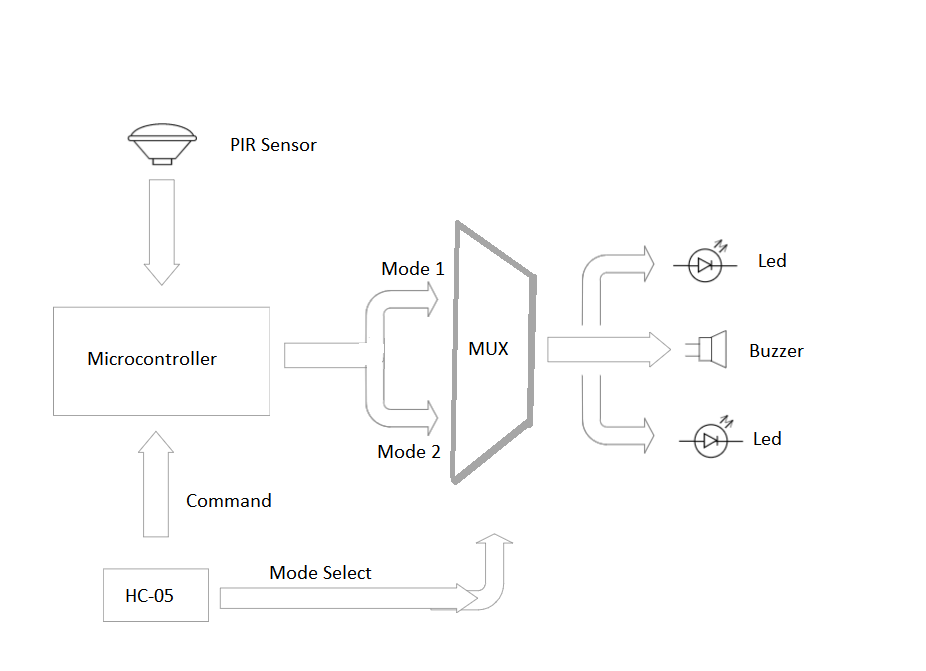
\includegraphics[width=1\textwidth]{fig/blockDiagram}
\caption{The block diagram of the alarm system}
\label{fig:fig1}

\end{figure}

The alarm system consists of a microcontroller, a PIR sensor for detecting motion, a HC-05 Bluetooth module for configuring the functionality of the system, and a buzzer and 2 LEDs .

The microcontroller takes inputs from the PIR sensor and from the Bluetooth module. Based on these inputs, it may send a signal to the Buzzer and the 2 leds. This signals depends on a variety of factors, such as if the alarm is turned on or which of the two modes is selected. These functionalities will be discussed in more detail in \autoref{chap:c3}

\section{Use cases}

This section discusses the way the user can interact with the alarm system, as seen in \autoref{fig:fig2}

\begin{figure}[h]

\centering
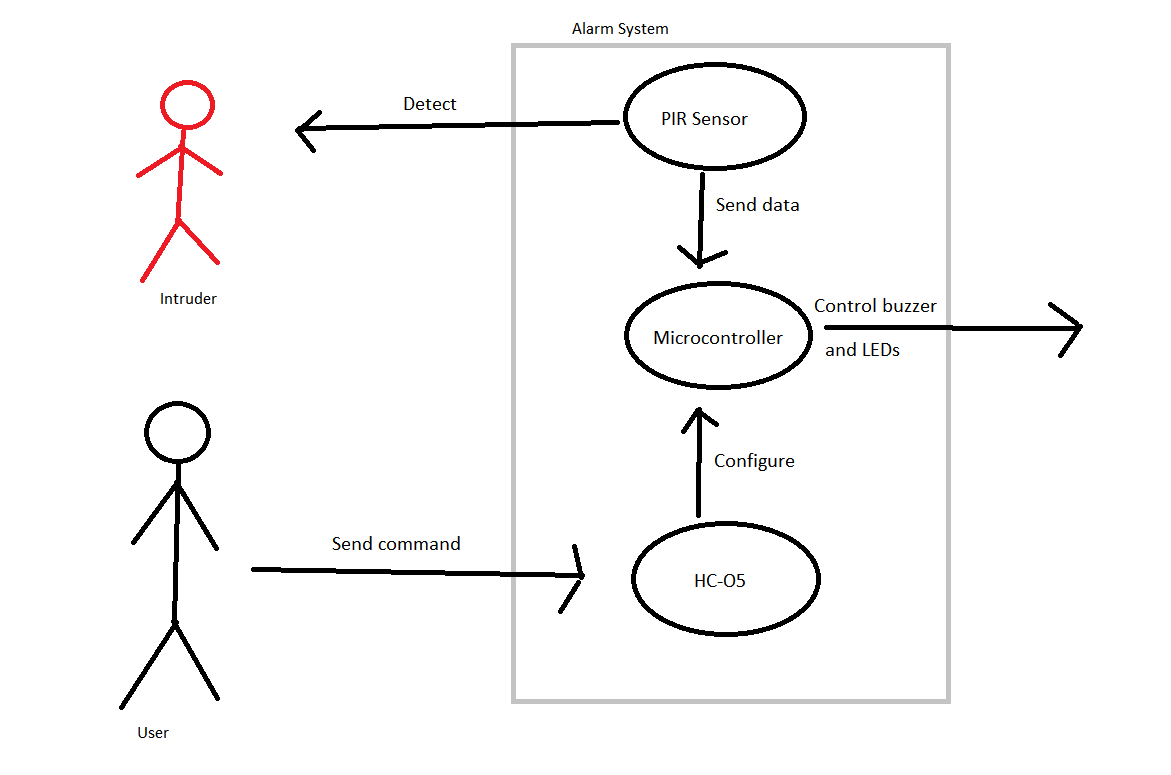
\includegraphics[width=1\textwidth]{fig/useCase}
\caption{The use case diagram of the alarm system}
\label{fig:fig2}

\end{figure}

The user can interact with the alarm system by sending commands through the Bluetooth module. The PIR sensor detects any motion, and sends its data to the Microcontroller, which depending on what configuration it got from the user, it controls the buzzer and the two LEDs.

\section{Communication protocol}

The project uses the \textbf{RS232} communication protocol (the UART interface through which it communicates with the Bluetooth module).
You can read more about this protocol \href{https://circuitdigest.com/article/rs232-serial-communication-protocol-basics-specifications}{here}.

\chapter{Detailed design and implementation}
\label{chap:c3}

\colorbox{blue!20}{\fbox{\begin{minipage}{1.0\textwidth}

This chapter will discuss in detail the design and implementation of the alarm system. It will analyze both the hardware and the software parts.

\end{minipage}}}

\section{Hardware}

The hardware design of the project can be seen in \autoref{fig:fig3}.

\vspace{5mm}

\begin{figure}[h]

\centering
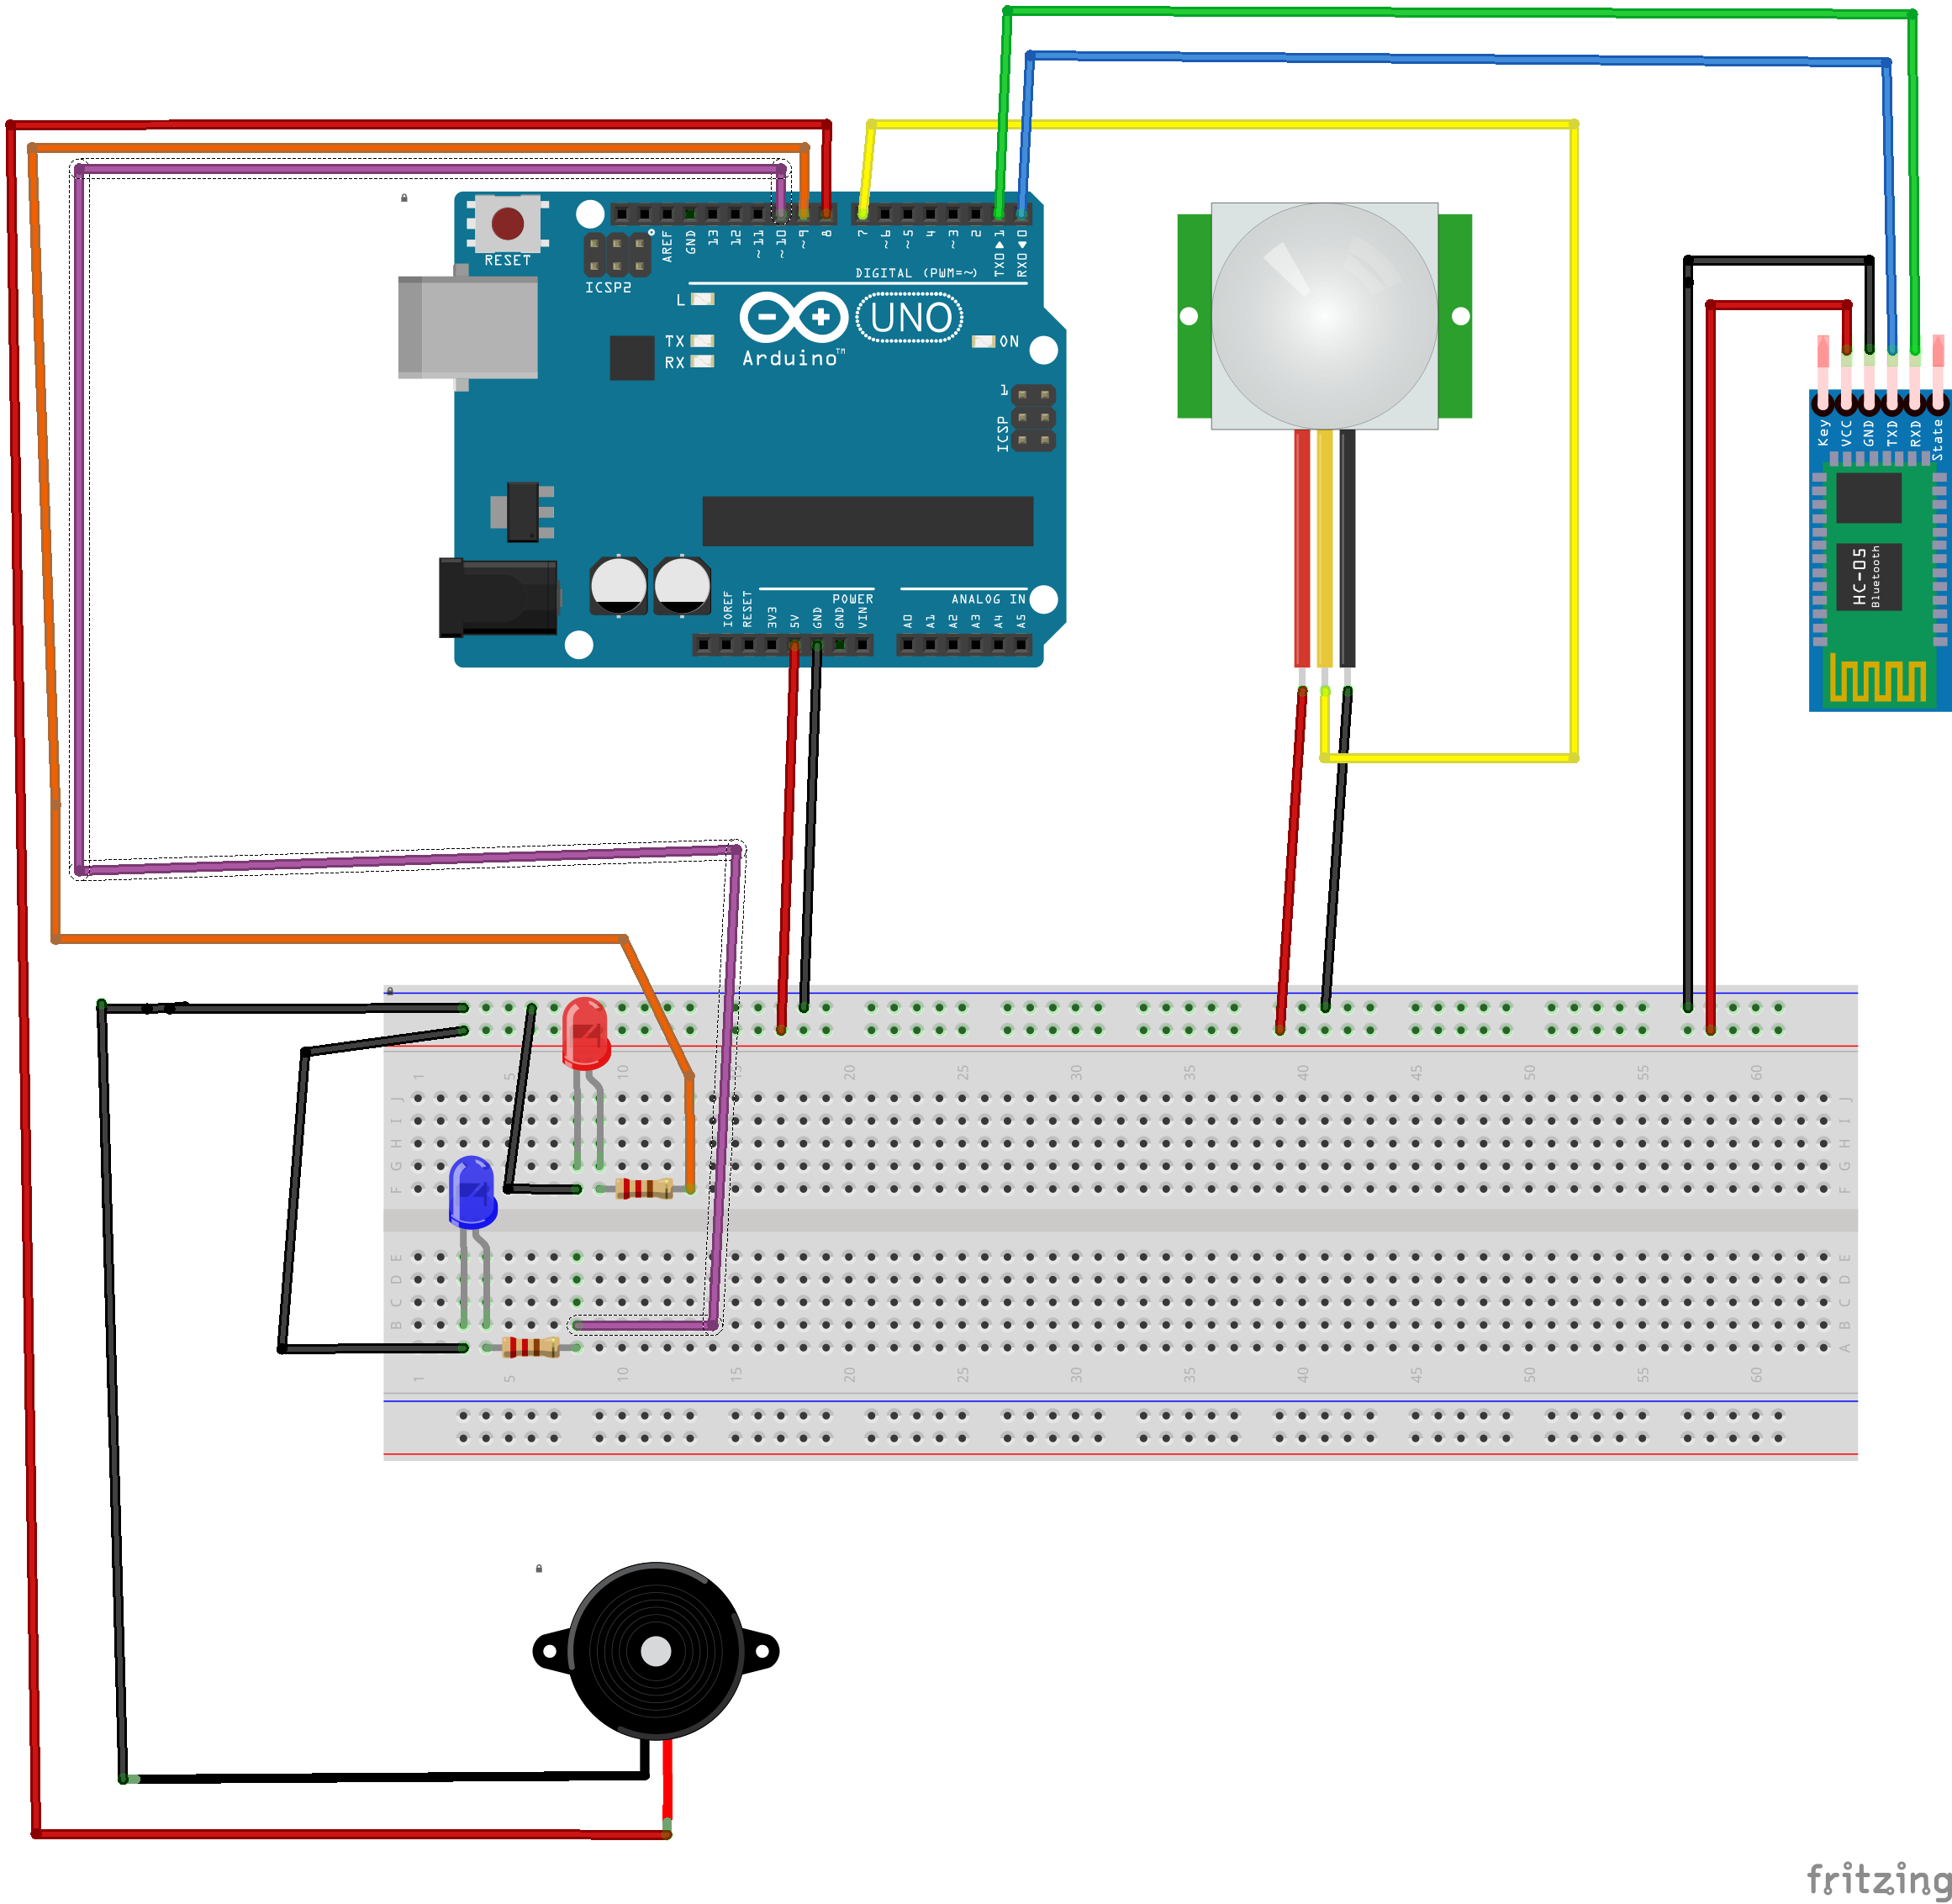
\includegraphics[scale=0.6]{fig/SchemaFritzing}
\caption{The hardware design of the alarm system}
\label{fig:fig3}

\end{figure}

\vspace{1cm}

The hardware components used in this project are:

\begin{itemize}

\item 1 x Arduino UNO microcontroller
\item 1 x PIR sensor
\item 1 x  HC-05 Bluetooth module
\item 2 x LEDs
\item 2 x \SI{220}{\ohm} resistors

\end{itemize}

\vspace{5mm}

\section{Software}

This section will discuss in detail the algorithms / functionalities that have been implemented.

\vspace{5mm}

The user needs to be able to communicate with the alarm system using the Bluetooth module, therefore a function which takes the input from the Bluetooth module and selects the appropriate action based on the input it received from the user 

\vspace{5mm}

The user needs to be able to:

\begin{itemize}

\item Arm the alarm system
\item Disarm the alarm system
\item Change the tone of the buzzer
\item Switch between the 2 modes of the alarm
\item Test the buzzer
\item Activate the \emph{"secret"} function 

\end{itemize}

\vspace{5mm}

The \textbf{arming/disarming} of the alarm is simple. If the alarm is \textbf{armed}, it detects responds to the input from the PIR senor, \textbf{otherwise} it does not. The user does this using the commands \emph{arm} and \emph{disarm}.

\vspace{5mm}

There are 3 distinct \textbf{tones} that are used. One is used for the first mode, and the other two for the second mode. The user can change those tones by using the commands \emph{tone, tone 1} or \emph{tone2}, followed by a space and a number representing the frequency. This frequency needs to be between \SI{100}{\hertz} and  \SI{3000}{\hertz}

\vspace{5mm}

The 2 \textbf{modes} of the application are as follows:

\begin{enumerate}

\item When the PIR sensor signals that it has detected something, the buzzer is on with the first tone, and the first led is on. When the PIR sensor goes from 1 to 0, the buzzer and the led turn off.
\item  When the PIR sensor is 1, the buzzer is on using the second tone and the first led is on. After half a second, the buzzer uses the third tone, the first led turns off and the second led turns on. This last for another half second. One second after the PIR section signaled it has detected something, the PIR sensor input is queried again to see whether the cycle starts again.

\end{enumerate}

\vspace{5mm}

When the user wants to \textbf{test} the buzzer, the buzzer will turn on and use the first tone for one second.

\vspace{5mm}

The \textbf{"secret"} function, when activated, uses the buzzer  to play a melody and controls the LEDs in time with the melody.

\chapter{Testing and validation}

The following actions have been taken when testing the application:

\begin{itemize}

\item Alarm has been disarmed to ensure the alarm doesn't go off when the sensor detects motion
\item Alarm has been armed and both modes have been tested, one at a time, to make sure the behavior of the buzzer and the two LEDs is the expected one
\item The test command has been given both in the \emph{armed} and \emph{disarmed} modes, to make sure the buzzer turns on
\item Tones have been changed to various valid values
\item Invalid tone values have been given to ensure the system responds with an error message
\item The secret command has been tested 


\end{itemize}

\vspace{5mm}

After testing the system, it has been established that the behavior is indeed the expected one.

\chapter{Conclusions}

This project offers an alarm system that can detect a intruder using a PIR sensor and warns the user with the help of a buzzer and two LEds.  The alarm system communicates with the user using a Bluetooth module, offering to the user the possibility to turn the alarm system on/off customize certain aspects of the system, such as changing the tone of the buzzer and switching between the two modes that the system offers.

\vspace{5mm}

The system offers a "secret" mode, which plays a melody. This mode is not relevant to the alrm system itself, but if nothing else, it can be used to test the buzzer's functionality with a wider range of frequencies and the functionality of the 2 LEDs.

\chapter{Bibliography}

\begin{enumerate}

\item \href{https://components101.com/sensors/hc-sr505-pir-sensor-pinout-datasheet}{HC-SR505 PIR Motion Sensor Module Datasheet}.
\item \href{https://components101.com/buzzer-pinout-working-datasheett}{Active Passive Buzzer Datasheet}.
\item \href{https://github.com/robsoncouto/arduino-songs/blob/master/nevergonnagiveyouup/nevergonnagiveyouup.ino}{The melody of the "secret" mode}.

\end{enumerate}


\chapter{Annex}

\begin{frame}

\lstset{language=C++,
                basicstyle=\ttfamily,
                keywordstyle=\color{blue}\ttfamily,
                stringstyle=\color{red}\ttfamily,
                commentstyle=\color{green}\ttfamily,
                morecomment=[l][\color{magenta}]{\#}
}
\begin{lstlisting}
   
#define NOTE_B0  31
#define NOTE_C1  33
#define NOTE_CS1 35
#define NOTE_D1  37
#define NOTE_DS1 39
#define NOTE_E1  41
#define NOTE_F1  44
#define NOTE_FS1 46
#define NOTE_G1  49
#define NOTE_GS1 52
#define NOTE_A1  55
#define NOTE_AS1 58
#define NOTE_B1  62
#define NOTE_C2  65
#define NOTE_CS2 69
#define NOTE_D2  73
#define NOTE_DS2 78
#define NOTE_E2  82
#define NOTE_F2  87
#define NOTE_FS2 93
#define NOTE_G2  98
#define NOTE_GS2 104
#define NOTE_A2  110
#define NOTE_AS2 117
#define NOTE_B2  123
#define NOTE_C3  131
#define NOTE_CS3 139
#define NOTE_D3  147
#define NOTE_DS3 156
#define NOTE_E3  165
#define NOTE_F3  175
#define NOTE_FS3 185
#define NOTE_G3  196
#define NOTE_GS3 208
#define NOTE_A3  220
#define NOTE_AS3 233
#define NOTE_B3  247
#define NOTE_C4  262
#define NOTE_CS4 277
#define NOTE_D4  294
#define NOTE_DS4 311
#define NOTE_E4  330
#define NOTE_F4  349
#define NOTE_FS4 370
#define NOTE_G4  392
#define NOTE_GS4 415
#define NOTE_A4  440
#define NOTE_AS4 466
#define NOTE_B4  494
#define NOTE_C5  523
#define NOTE_CS5 554
#define NOTE_D5  587
#define NOTE_DS5 622
#define NOTE_E5  659
#define NOTE_F5  698
#define NOTE_FS5 740
#define NOTE_G5  784
#define NOTE_GS5 831
#define NOTE_A5  880
#define NOTE_AS5 932
#define NOTE_B5  988
#define NOTE_C6  1047
#define NOTE_CS6 1109
#define NOTE_D6  1175
#define NOTE_DS6 1245
#define NOTE_E6  1319
#define NOTE_F6  1397
#define NOTE_FS6 1480
#define NOTE_G6  1568
#define NOTE_GS6 1661
#define NOTE_A6  1760
#define NOTE_AS6 1865
#define NOTE_B6  1976
#define NOTE_C7  2093
#define NOTE_CS7 2217
#define NOTE_D7  2349
#define NOTE_DS7 2489
#define NOTE_E7  2637
#define NOTE_F7  2794
#define NOTE_FS7 2960
#define NOTE_G7  3136
#define NOTE_GS7 3322
#define NOTE_A7  3520
#define NOTE_AS7 3729
#define NOTE_B7  3951
#define NOTE_C8  4186
#define NOTE_CS8 4435
#define NOTE_D8  4699
#define NOTE_DS8 4978
#define REST      0

// change this to make the song slower or faster
int tempo = 114;

int melody[] = {

  NOTE_D5, 2, NOTE_E5, 8, NOTE_FS5, 8, NOTE_D5, 8, //13
  NOTE_E5, 8, NOTE_E5, 8, NOTE_E5, 8, NOTE_FS5, 8, 
NOTE_E5, 4, NOTE_A4, 4,
  REST, 2, NOTE_B4, 8, NOTE_CS5, 8, NOTE_D5, 8, NOTE_B4, 8,
  REST, 8, NOTE_E5, 8, NOTE_FS5, 8, NOTE_E5, -4, NOTE_A4, 16, NOTE_B4, 
16, NOTE_D5, 16, NOTE_B4, 16,
  NOTE_FS5, -8, NOTE_FS5, -8, NOTE_E5, -4, NOTE_A4, 16, 
NOTE_B4, 16, NOTE_D5, 16, NOTE_B4, 16,

  NOTE_E5, -8, NOTE_E5, -8, NOTE_D5, -8, NOTE_CS5, 
16, NOTE_B4, -8, NOTE_A4, 16, NOTE_B4, 16, NOTE_D5, 16, NOTE_B4, 16, //18
  NOTE_D5, 4, NOTE_E5, 8, NOTE_CS5, -8, NOTE_B4, 16,
 NOTE_A4, 8, NOTE_A4, 8, NOTE_A4, 8,
  NOTE_E5, 4, NOTE_D5, 2, NOTE_A4, 16, 
NOTE_B4, 16, NOTE_D5, 16, NOTE_B4, 16,
  NOTE_FS5, -8, NOTE_FS5, -8, NOTE_E5, -4,
 NOTE_A4, 16, NOTE_B4, 16, NOTE_D5, 16, NOTE_B4, 16,
  NOTE_A5, 4, NOTE_CS5, 8, NOTE_D5, -8, NOTE_CS5, 
16, NOTE_B4, 8, NOTE_A4, 16, NOTE_B4, 16, NOTE_D5, 16, NOTE_B4, 16,

  NOTE_D5, 4, NOTE_E5, 8, NOTE_CS5, -8, NOTE_B4, 16,
 NOTE_A4, 4, NOTE_A4, 8, //23
  NOTE_E5, 4, NOTE_D5, 2, REST, 4
};

// sizeof gives the number of bytes, each int value is composed of
// two bytes (16 bits)
// there are two values per note (pitch and duration), 
//so for each note there are four bytes
int notes = sizeof(melody) / sizeof(melody[0]) / 2;

// this calculates the duration of a whole note in ms
int wholenote = (60000 * 4) / tempo;

int divider = 0, noteDuration = 0;





int PIR = 7;
int buzzerPin = 8;
int pinLed1 = 9;
int pinLed2 = 10;
int detection;

int tone0;
int tone1;
int tone2;

String command = "";
bool commandDone = false;
bool normalMode = true;
bool armed;

void setup() {

  pinMode(PIR, INPUT);
  pinMode(buzzerPin, OUTPUT);
  pinMode(pinLed1, OUTPUT);
  pinMode(pinLed2, OUTPUT);

  Serial.begin(9600);
  Serial.setTimeout(100);
  armed = false;

  tone0 = 500;
  tone1 = 500;
  tone2 = 600;

}

void loop() {

  if (commandDone == true)
    handleCommand();

  if (armed)
  {

    detection = digitalRead(PIR);
    //Serial.println(detection);
    if (normalMode)
    {

      if (detection == HIGH)
      {
        tone(buzzerPin, tone0);
        digitalWrite(pinLed1, HIGH);
        digitalWrite(pinLed2, LOW);
      }
      else
      {
        noTone(buzzerPin);
        digitalWrite(pinLed1, LOW);
        digitalWrite(pinLed2, LOW);
      }
    }
    else
    {
      if (detection == HIGH)
      {
        tone(buzzerPin, tone1);
        digitalWrite(pinLed1, HIGH);
        digitalWrite(pinLed2, LOW);
        delay(500);
        noTone(buzzerPin);

        tone(buzzerPin, tone2, 1000);
        digitalWrite(pinLed1, LOW);
        digitalWrite(pinLed2, HIGH);
        delay(500);
        noTone(buzzerPin);

        digitalWrite(pinLed1, LOW);
        digitalWrite(pinLed2, LOW);
      }
      // else noTone(buzzerPin);
    }

  }
  else
  {
    noTone(buzzerPin);
    digitalWrite(pinLed1, LOW);
    digitalWrite(pinLed2, LOW);
  }



}

void beep(int pin, int times, int pinLed)
{
  digitalWrite(pinLed1, LOW);
  digitalWrite(pinLed2, LOW);
  
  noTone(pin);
  delay(100);
  for (int i = 0; i < times; i++)
  {
    tone(pin, 700);
    digitalWrite(pinLed, HIGH);
    delay(200);
    noTone(pin);
    digitalWrite(pinLed, LOW);
    delay(50);
    
  }
}

void handleSecretCommand()
{
  bool redLight = true;
  // iterate over the notes of the melody.
  // Remember, the array is twice the number of notes (notes + durations)
  for (int thisNote = 0; thisNote < notes * 2; thisNote = thisNote + 2) {

    // calculates the duration of each note
    divider = melody[thisNote + 1];
    if (divider > 0) {
      // regular note, just proceed
      noteDuration = (wholenote) / divider;
    } else if (divider < 0) {
      // dotted notes are represented with negative durations!!
      noteDuration = (wholenote) / abs(divider);
      noteDuration *= 1.5; // increases the duration in half for
					// dotted notes
    }

     if(melody[thisNote] != REST)
     {
      
        if(redLight)
        {
            digitalWrite(pinLed1, HIGH);
            digitalWrite(pinLed2, LOW);
        }
        else
        {
            digitalWrite(pinLed1, LOW);
            digitalWrite(pinLed2, HIGH);
        }
        redLight = !redLight;
     }
     else
     {
        digitalWrite(pinLed1, LOW);
        digitalWrite(pinLed2, LOW);
     }
      
     // we only play the note for 90% of the duration, leaving 10% as a pause
    tone(buzzerPin, melody[thisNote], noteDuration * 0.9);

    // Wait for the specief duration before playing the next note.
    delay(noteDuration);

    // stop the waveform generation before the next note.
    noTone(buzzerPin);

   
      


  }
    digitalWrite(pinLed1, LOW);
    digitalWrite(pinLed2, LOW);
}

void handleToneCommand()
{
  int toneVal = 0;
  int i;

  bool change0 = false;
  bool change1 = false;
  bool change2 = false;


  if (command[4] == ' ')
  {
    change0 = true;
    i = 5;
  }
  else if (command[4] == '1')
  {
    change1 = true;
    i = 6;
  }
  else if (command[4] == '2')
  {
    change2 = true;
    i = 6;
  }
  else
  {
    Serial.println("Invalid 'tone' command");
    return;
  }

  while (command[i] >= '0' && command[i] <= '9')
  {
    toneVal = toneVal * 10 + (command[i] - '0');

    i++;
  }

  Serial.print("Tone is ");
  Serial.println(toneVal);

  if (toneVal < 100 || toneVal > 3000)
    Serial.println("Error: Tone value has to be between 100 and 3000");
  else
  {
    if (change0)
      tone0 = toneVal;

    if (change1)
      tone1 = toneVal;

    if (change2)
      tone2 = toneVal;

  }


}

void handleCommand()
{
  bool validCommand = false;

  Serial.println("Handling command: " + command);



  if (command.equals("arm") || command.equals("arm\n") 
|| command.equals("arm\n\n"))
  {
    Serial.println("Arming");

    beep(buzzerPin, 3, pinLed1);

    armed = true;

    validCommand = true;
  }



  if (command.equals("disarm") || command.equals("disarm\n")
 || command.equals("disarm\n\n"))
  {
    Serial.println("Disarming");

    beep(buzzerPin, 2, pinLed1);

    armed = false;

    validCommand = true;
  }

  if (command.indexOf("tone") == 0)
  {
    handleToneCommand();

    validCommand = true;
  }

  if (command.equals("mode1") || command.equals("mode1\n")
 || command.equals("mode1\n\n"))
  {
    Serial.println("Mode 1 : Active");
    normalMode = true;

    beep(buzzerPin, 2, pinLed2);

    validCommand = true;
  }

  if (command.equals("mode2") || command.equals("mode2\n")
 || command.equals("mode2\n\n"))
  {
    Serial.println("Mode 2 : Active");
    normalMode = false;

     beep(buzzerPin, 3, pinLed2);
    
    validCommand = true;
  }

  if (command.equals("test") || command.equals("test\n")
 || command.equals("test\n\n"))
  {
    tone(buzzerPin, tone0);
    delay(1000);

    validCommand = true;
  }

  if (command.equals("secret") || command.equals("secret\n") 
|| command.equals("secret\n\n"))
  {
    handleSecretCommand();

    validCommand = true;
  }

  commandDone = false;
  command = "";

  if (!validCommand)
    Serial.println("Invalid command");

}

void serialEvent()
{
  command = Serial.readString();
  delay(100);
  //command += '\n';
  command += '\0';
  commandDone = true;
}

\end{lstlisting}
\end{frame}

\end{document}